
%!TEX root = ../main.tex


\section{Entity-Relationship (E-R) Model}

\subsection{Introduction to the Entity-Relationship (E-R) Model}
Before writing SQL code or creating tables, we must understand the data we are trying to organize. To do this, we use the \textbf{Entity-Relationship (E-R) Model}.

\begin{defbox}{Entity-Relationship Model}
A conceptual data model used to formally represent the structure, objects, and rules of a real-world domain, completely independent of how the data will physically be stored.
\end{defbox}

\subsubsection{The E-R Model in Database Design}
Database design is a multi-step process. The E-R model belongs strictly to the first phase.

\begin{enumerate}
    \item \textbf{Conceptual Design} (Where E-R lives): Describing the reality of interest at a high level. No tables, no SQL, no storage constraints. Just abstract logic and meaning.
    \item \textbf{Logical Design:} Transforming the conceptual E-R schema into a relational schema (tables, foreign keys).
    \item \textbf{Physical Design:} Implementing the logical schema into a specific DBMS (e.g., PostgreSQL, Oracle), dealing with indexes, hardware, and performance.
\end{enumerate}

         \begin{figure}[H] 
        \centering
\includegraphics[scale=0.55]{6.E-R model.jpg}
        \caption{E-R model}
    \captionsetup{font=footnotesize}
    \end{figure}

\subsubsection{Main Constructs of the E-R Model}
To describe a complex reality, the E-R model provides a small but powerful set of modeling tools called \textbf{constructs}.

\begin{defbox}{Construct}
A basic modeling element used in the E-R model to formally describe an aspect of the real world.
\end{defbox}

The three primary structural constructs are:

\pagebreak
\begin{enumerate}
\item \textbf{Entity}

A class of objects in the application domain (people, things, events) that share common properties and have an autonomous, independent existence.


\vspace{0.2cm}
\begin{example}{\textbf{Example: Entity}}

In a university database, \texttt{STUDENT}, \texttt{COURSE}, and \texttt{PROFESSOR} are all Entities.
\end{example}

\vs
\item \textbf{Relationship}

A logical and meaningful link between two or more entities.


\vspace{0.2cm}
\begin{example}{\textbf{Example: Relationship}}

\texttt{STUDENT} and \texttt{COURSE} are entities. The action \texttt{"Enrolls\_In"} is the Relationship connecting them.
\end{example}

\vs
\item \textbf{Attribute}

An elementary property used to describe an Entity or a Relationship.

\vspace{0.2cm}
\begin{example}{\textbf{Example: Attribute}}

For the \texttt{STUDENT} entity, attributes would be \texttt{Name}, \texttt{Surname}, and \texttt{DateOfBirth}. \\
Interestingly, the relationship \texttt{"Enrolls\_In"} can also have an attribute, such as \texttt{EnrollmentDate}.
\end{example}
\end{enumerate}


\subsubsection{Constraints in the E-R Model}
While Entities, Relationships, and Attributes describe the \textit{structure} of the data, the model also needs to enforce the \textit{rules} of reality. 

While often listed as constructs, the following two concepts are technically \textbf{Integrity Constraints} applied to the building blocks above.

\begin{defbox}{Relationship Cardinality}
A constraint (usually expressed as a min/max pair) that dictates how many times a specific entity occurrence can participate in a relationship.
\end{defbox}

\vspace{0.2cm}
\begin{example}{\textbf{Example: Cardinality}}

A \texttt{STUDENT} can enroll in many \texttt{COURSES}, but must be enrolled in at least one. The cardinality is \textbf{(1, N)}.
\end{example}

\begin{defbox}{Entity Identifier}
An attribute, or set of attributes, that uniquely distinguishes one occurrence of an entity from all other occurrences of that same entity. (This is the conceptual equivalent of a Primary Key).
\end{defbox}

\vspace{0.2cm}
\begin{example}{\textbf{Example: Identifier}}
  
For the \texttt{STUDENT} entity, the \texttt{Name} is not a valid identifier (two students can be named Mario). The \texttt{StudentID} (Matricola) is the perfect identifier.
\end{example}
\subsection{Introduction to Entities, Relationships, and Attributes}

The Entity-Relationship (E-R) model simplifies the real world into three foundational building blocks: \textbf{Entities}, \textbf{Relationships}, and \textbf{Attributes}. This model allows us to visually and logically map out a domain before we ever write a line of SQL.

\begin{defbox}{E-R Model}
A conceptual modeling technique that represents a real-world domain by identifying the key objects (entities), their properties (attributes), and how they interact (relationships).
\end{defbox}

\subsubsection{Entities and Their Occurrences}

\begin{defbox}{Entity}
A broad class or category of objects (people, places, things, concepts) within the application domain that share common properties and exist independently.
\end{defbox}

An entity represents a \textit{type} of thing, not the thing itself.
\begin{itemize}
    \item \textbf{Good Entity Names:} \texttt{Student}, \texttt{City}, \texttt{Invoice}.
    \item \textbf{Naming Convention:} Use singular nouns. A singular noun emphasizes that the entity is a template or class.
    \item \textbf{Graphical Representation:} Drawn as a \textbf{Rectangle}.
\end{itemize}

\begin{center}
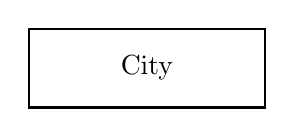
\begin{tikzpicture}
  \node[draw, rectangle, minimum width=3cm, minimum height=1cm, thick] {City};
\end{tikzpicture}
\end{center}


\subsubsection{Entity vs. Occurrence (Instance)}
It is critical to distinguish between the abstract category and the actual physical data.

\begin{defbox}{Entity Occurrence (Instance)}
One specific, individual object that belongs to the class defined by the entity. 
\end{defbox}

\vspace{0.2cm}
\begin{example}{\textbf{Example: Entity vs. Occurrence}}


\vspace{0.2cm}
\begin{center}
\begin{tabular}{|l|l|}
\hline
\textbf{Conceptual Entity (The Class)} & \textbf{Physical Occurrence (The Instance)} \\
\hline
\texttt{City} & Naples, Rome, Milan \\
\texttt{Employee} & Mario Rossi, Luigi Bianchi \\
\texttt{Department} & Sales, IT, Human Resources \\
\hline
\end{tabular}
\end{center}
\textit{Note: In an E-R diagram, you only draw the Entity (City), you never draw the occurrences (Naples).}
\end{example}

\subsubsection{Relationships and Their Occurrences}

\begin{defbox}{Relationship}
A meaningful logical association or link connecting two or more entities.
\end{defbox}

While entities are the "nouns" of your database, relationships describe how those nouns interact.
\begin{itemize}
    \item \textbf{Naming Convention:} Usually a singular noun (e.g., \texttt{Enrollment}, \texttt{Affiliation}) rather than a verb, to avoid implying a one-way direction. 
    \item \textbf{Graphical Representation:} Drawn as a \textbf{Diamond}.
\end{itemize}

\subsubsection{Relationship Occurrences}
Just as entities have instances, relationships do too.

\begin{defbox}{Relationship Occurrence}
A specific, mathematical pairing (or tuple) of entity occurrences that are linked together. The E-R model strictly dictates that \textbf{repeated identical occurrences are not allowed} within the same relationship.
\end{defbox}

\vspace{0.2cm}
\begin{example}{\textbf{Example: Relationship Occurrences}}



\vspace{0.2cm}
Entities: \texttt{Employee} and \texttt{Department}.\\
Relationship: \texttt{Affiliation}.\\
Occurrence: \textit{(Mario Rossi, IT Department)}.

\vs

\begin{center}
\begin{tikzpicture}
  \node[draw, rectangle, minimum width=2.5cm, minimum height=1cm, thick] (emp) at (0,0) {Employee};
  \node[draw, diamond, aspect=2, minimum width=2.5cm, minimum height=1cm, thick] (aff) at (4,0) {Affiliation};
  \node[draw, rectangle, minimum width=2.5cm, minimum height=1cm, thick] (dept) at (8,0) {Department};
  \draw[thick] (emp) -- (aff);
  \draw[thick] (aff) -- (dept);
\end{tikzpicture}
\end{center}

\end{example}

\subsection{Complex Relationships: N-ary and Recursive}
Relationships are not always simple one-to-one or one-to-many links between two distinct entities.

\subsubsection{N-ary Relationships}
Most relationships are binary (connecting 2 entities). However, some scenarios require connecting 3 or more entities simultaneously.

\begin{defbox}{N-ary Relationship}
A relationship that involves $n$ participating entities in a single, indivisible logical link.
\end{defbox}

\vspace{0.2cm}
\begin{example}{\textbf{Example: Ternary Relationship}}



\vspace{0.2cm}
Relationship: \texttt{Supply}.\\
Involved Entities: \texttt{Supplier}, \texttt{Product}, \texttt{Department}.\\
Meaning: Supplier A provides Product B specifically to Department C. This cannot be broken down into binary relationships without losing the context that \textit{this specific supplier gave this specific product to this specific department}.

\vs

\begin{center}
\begin{tikzpicture}
  \node[draw, diamond, aspect=2, minimum width=2.5cm, minimum height=1cm, thick] (supply) at (0,0) {Supply};
  \node[draw, rectangle, minimum width=2.5cm, minimum height=1cm, thick] (supplier) at (-4,0) {Supplier};
  \node[draw, rectangle, minimum width=2.5cm, minimum height=1cm, thick] (product) at (4,0) {Product};
  \node[draw, rectangle, minimum width=2.5cm, minimum height=1cm, thick] (dept) at (0,-2.5) {Department};
  \draw[thick] (supplier) -- (supply);
  \draw[thick] (product) -- (supply);
  \draw[thick] (dept) -- (supply);
\end{tikzpicture}
\end{center}
\end{example}

\subsubsection{Recursive Relationships and Roles}
Sometimes, an entity needs to have a relationship with itself.

\begin{defbox}{Recursive Relationship}
A relationship where the same entity participates more than once.
\end{defbox}

\vspace{0.2cm}
\begin{example}{\textbf{Example: Symmetric Recursive}}



\vspace{0.2cm}
Entity: \texttt{Employee}.\\
Relationship: \texttt{Colleague}.\\
Mario is a colleague of Luigi. The relationship is symmetric; both participate equally as colleagues.

\vs

\begin{center}
\begin{tikzpicture}
  \node[draw, rectangle, minimum width=2.5cm, minimum height=1cm, thick] (emp) at (0,0) {Employee};
  \node[draw, diamond, aspect=2, minimum width=2.5cm, minimum height=1cm, thick] (colleague) at (4,0) {Colleague};
  \draw[thick] (emp.north) -- ++(0,0.8) -| (colleague.north);
  \draw[thick] (emp.south) -- ++(0,-0.8) -| (colleague.south);
\end{tikzpicture}
\end{center}
\end{example}

If a recursive relationship is \textbf{asymmetric} (directional), we must define \textbf{Roles} to clarify who is doing what.

\begin{defbox}{Role}
A label specifying the distinct function played by an entity occurrence within a relationship.
\end{defbox}

\vspace{0.2cm}
\begin{example}{\textbf{Example: Asymmetric Recursive with Roles}}


    
\vspace{0.2cm}
Entity: \texttt{Employee}.\\
Relationship: \texttt{Supervision}.\\
Because supervision implies a hierarchy, we must label the lines connecting the entity to the diamond:\\
- Line 1 Role: \textbf{Manager}\\
- Line 2 Role: \textbf{Subordinate}\\
This clarifies that Mario (Manager) supervises Luigi (Subordinate).

\vs

\begin{center}
\begin{tikzpicture}
  \node[draw, rectangle, minimum width=2.5cm, minimum height=1cm, thick] (emp) at (0,0) {Employee};
  \node[draw, diamond, aspect=2, minimum width=2.5cm, minimum height=1cm, thick] (sup) at (5,0) {Supervision};
  \draw[thick] (emp.north) -- ++(0,1) -| node[pos=0.25, above, font=\small] {Manager} (sup.north);
  \draw[thick] (emp.south) -- ++(0,-1) -| node[pos=0.25, below, font=\small] {Subordinate} (sup.south);
\end{tikzpicture}
\end{center}
\end{example}

\subsection{Cardinality of Relationships}
Knowing that two entities are connected is not enough. To build an accurate database, we must explicitly define \textbf{how many times} an entity occurrence can participate in that connection.

\begin{defbox}{Relationship Cardinality}
A pair of values $(min, max)$ associated with each entity participating in a relationship. These values specify the minimum and maximum number of occurrences an entity instance is allowed to participate in.
\end{defbox}

The $(min, max)$ pair answers two distinct questions:
\begin{enumerate}
    \item \textbf{Minimum:} Is participation optional (0) or mandatory (1)?
    \item \textbf{Maximum:} Can it only happen once (1) or multiple times (N)?
\end{enumerate}

\subsubsection{Allowed Values for Cardinalities}
While any non-negative integer is technically allowed as long as $min \leq max$, the E-R model simplifies this to three standard symbols: \textbf{0, 1, and N} (meaning "many" or "unbounded").

\begin{center}
\begin{tabular}{|c|l|}
\hline
\textbf{Cardinality} & \textbf{Meaning in plain English} \\
\hline
$(0,1)$ & Optional participation, but if it happens, at most one time. \\
$(1,1)$ & Mandatory participation, and exactly one time. \\
$(0,N)$ & Optional participation, but can happen many times. \\
$(1,N)$ & Mandatory participation, must happen at least once, but can happen many times. \\
\hline
\end{tabular}
\end{center}

\vspace{0.2cm}
\begin{example}{\textbf{Example: Employee-Department Cardinality}}

    \vs

\begin{itemize}
    \item The $(1,1)$ next to \texttt{Employee} means: An employee \textbf{must} belong to a department (min 1), and can belong to \textbf{only one} department (max 1).
    \item The $(1,N)$ next to \texttt{Department} means: A department \textbf{must} have at least one employee (min 1) and can have \textbf{many} employees (max N).
\end{itemize}

\vs
\begin{center}
\begin{tikzpicture}
  \node[draw, rectangle, minimum width=2.5cm, minimum height=1cm, thick] (emp) at (0,0) {Employee};
  \node[draw, diamond, aspect=2, minimum width=2.5cm, minimum height=1cm, thick] (aff) at (4,0) {Affiliation};
  \node[draw, rectangle, minimum width=2.5cm, minimum height=1cm, thick] (dept) at (8,0) {Department};
  
  \draw[thick] (emp) -- node[above] {(1,1)} (aff);
  \draw[thick] (aff) -- node[above] {(1,N)} (dept);
\end{tikzpicture}
\end{center}

\end{example}

\subsubsection{Types of Relationships (Based on Maximum Cardinality)}
By looking \textit{only} at the Maximum values on both sides of the relationship, we can classify the entire relationship into one of three structural types.


\begin{defbox}{Many-to-Many (N:N)}
A relationship where both entities have a maximum cardinality of $N$.
\end{defbox}

\vspace{0.2cm}
\begin{example}{\textbf{Example: Many-to-Many}}

    \vs
\begin{center}
\begin{tikzpicture}
  \node[draw, rectangle, minimum width=2cm, minimum height=1cm, thick] (stu) at (0,0) {Student};
  \node[draw, diamond, aspect=2, minimum width=2.5cm, minimum height=1cm, thick] (exam) at (4,0) {Takes};
  \node[draw, rectangle, minimum width=2cm, minimum height=1cm, thick] (course) at (8,0) {Course};
  
  \draw[thick] (stu) -- node[above] {(0,N)} (exam);
  \draw[thick] (exam) -- node[above] {(0,N)} (course);
\end{tikzpicture}
\end{center}
A student can take \textbf{many} courses, and a course can be taken by \textbf{many} students.
\end{example}


\begin{defbox}{One-to-Many (1:N)}
A relationship where one entity has a maximum cardinality of $1$, and the other has a maximum cardinality of $N$.
\end{defbox}
\textit{Note: Direction matters here! It is crucial to identify which side is the "One" and which is the "Many".}

\vspace{0.2cm}
\begin{example}{\textbf{Example: One-to-Many}}

    \vs
\begin{center}
\begin{tikzpicture}
  \node[draw, rectangle, minimum width=2.5cm, minimum height=1cm, thick] (mun) at (0,0) {Municipality};
  \node[draw, diamond, aspect=2, minimum width=2.5cm, minimum height=1cm, thick] (loc) at (4,0) {Located In};
  \node[draw, rectangle, minimum width=2.5cm, minimum height=1cm, thick] (prov) at (8,0) {Province};
  
  \draw[thick] (mun) -- node[above] {(1,1)} (loc);
  \draw[thick] (loc) -- node[above] {(1,N)} (prov);
\end{tikzpicture}
\end{center}
A municipality belongs to exactly \textbf{one} province (max 1), but a province contains \textbf{many} municipalities (max N).
\end{example}

\pagebreak

\begin{defbox}{One-to-One (1:1)}
A relationship where both entities have a maximum cardinality of $1$.
\end{defbox}

\vspace{0.2cm}
\begin{example}{\textbf{Example: One-to-One}}

    \vs
\begin{center}
\begin{tikzpicture}
  \node[draw, rectangle, minimum width=2.5cm, minimum height=1cm, thick] (prof) at (0,0) {Tenured Prof.};
  \node[draw, diamond, aspect=2, minimum width=2.5cm, minimum height=1cm, thick] (own) at (4,0) {Owns};
  \node[draw, rectangle, minimum width=2.5cm, minimum height=1cm, thick] (chair) at (8,0) {Chair};
  
  \draw[thick] (prof) -- node[above] {(1,1)} (own);
  \draw[thick] (own) -- node[above] {(0,1)} (chair);
\end{tikzpicture}
\end{center}
Every tenured professor owns exactly \textbf{one} chair (max 1), and every chair is owned by at most \textbf{one} professor (max 1).
\end{example}

\subsection{Attributes and Their Classification}

In the E-R model, entities and relationships are described through \textbf{attributes}. Attributes are the elementary properties that give useful information about the objects or associations in the domain.

\begin{defbox}{Attribute}
An \textbf{attribute} is an elementary property of an entity or of a relationship that is relevant for the application domain.
\end{defbox}

Attributes are not exclusive to entities; they can also describe relationships.

\vspace{0.2cm}
\begin{example}{\textbf{Example: Entity Attribute vs Relationship Attribute}}

    In this university model, \texttt{Name} describes an object (the entity \texttt{Student}), while \texttt{Grade} describes the connection between objects (the relationship \texttt{Exam}).

\vspace{0.2cm}
\begin{center}
\begin{tikzpicture}[node distance=2cm, every node/.style={font=\small}]
  \node[draw, rectangle, minimum width=2cm, minimum height=1cm, thick] (stu) at (0,0) {Student};
  \node[draw, ellipse, inner sep=2pt] (name) at (-1.5,1.5) {Name};
  
  \node[draw, diamond, aspect=2, minimum width=2cm, minimum height=1cm, thick] (exam) at (4,0) {Exam};
  \node[draw, ellipse, inner sep=2pt] (grade) at (4,1.5) {Grade};
  
  \node[draw, rectangle, minimum width=2cm, minimum height=1cm, thick] (course) at (8,0) {Course};

  \draw[thick] (stu) -- (name);
  \draw[thick] (stu) -- (exam);
  \draw[thick] (exam) -- (course);
  \draw[thick] (exam) -- (grade);
\end{tikzpicture}
\end{center}

\end{example}

\subsubsection{Domain of an Attribute}
An attribute cannot take arbitrary values.

\begin{defbox}{Domain of an Attribute}
The \textbf{domain} of an attribute is the set of all admissible values that the attribute can assume.
\end{defbox}

The domain defines both the \textbf{data type} (e.g., string, integer) and the \textbf{valid range} (e.g., integers between 18 and 25).

\vs
\begin{center}
\begin{tabular}{|l|l|}
\hline
\textbf{Attribute} & \textbf{Possible Domain} \\
\hline
Surname & Strings of up to 20 characters \\
Age & Integers from 18 to 65 \\
\hline
\end{tabular}
\end{center}

\subsubsection{Composite vs. Simple Attributes}
Not all attributes are single, indivisible values.

\begin{itemize}
    \item \textbf{Simple Attribute}: 
an attribute that cannot be decomposed into smaller, meaningful sub-parts. (e.g., \texttt{Name}).

\vs

\item \textbf{Composite Attribute}: 
 group of attributes belonging to the same entity or relationship that are closely related in meaning or use, bundled together under a single parent attribute.
\end{itemize}



\vspace{0.2cm}
\begin{example}{\textbf{Example: Graphical Representation of Attributes}}

    In this university model, \texttt{Name} describes an object (the entity \texttt{Student}), while \texttt{Grade} describes the connection between objects (the relationship \texttt{Exam}).
\vspace{0.2cm}

\begin{center}
\begin{tikzpicture}[every node/.style={font=\small}]
  \node[draw, rectangle, minimum width=2.5cm, minimum height=1cm, thick] (emp) at (0,0) {Employee};
  
  % Simple Attributes
  \node[draw, ellipse, inner sep=2pt] (name) at (-2,1.5) {Name};
  \node[draw, ellipse, inner sep=2pt] (age) at (0,1.5) {Age};
  
  % Composite Attribute
  \node[draw, ellipse, inner sep=2pt] (address) at (3,1.5) {Address};
  \node[draw, ellipse, inner sep=2pt] (street) at (2,3) {Street};
  \node[draw, ellipse, inner sep=2pt] (num) at (4,3) {Number};

  \draw[thick] (emp) -- (name);
  \draw[thick] (emp) -- (age);
  \draw[thick] (emp) -- (address);
  \draw[thick] (address) -- (street);
  \draw[thick] (address) -- (num);
\end{tikzpicture}
\end{center}

\vs
Here, \texttt{Name} and \texttt{Age} are simple attributes. \texttt{Address} is a composite attribute decomposed into \texttt{Street} and \texttt{Number}.
\end{example}

\subsubsection{Cardinality of Attributes}
Just as relationships have cardinalities, attributes do too. Attribute cardinality defines how many values a single attribute can hold for a single entity occurrence.

\begin{defbox}{Attribute Cardinality}
A $(min, max)$ pair describing the minimum and maximum number of values that an attribute may assume for a single occurrence of an entity or relationship.
\end{defbox}

\textit{Note: If an attribute's cardinality is $(1,1)$, it is considered standard and is usually omitted from the E-R diagram.}

\vspace{0.3cm}
\begin{center}
\begin{tabular}{|c|l|l|}
\hline
\textbf{Cardinality} & \textbf{Type} & \textbf{Meaning} \\
\hline
$(1,1)$ & Mandatory & Must have exactly one value (Default). \\
$(0,1)$ & Optional & May have no value, or at most one. \\
$(0,N)$ & Multivalued (Opt) & May have zero, one, or many values. \\
$(1,N)$ & Multivalued (Mand) & Must have at least one value, but can have many. \\
\hline
\end{tabular}
\end{center}

\vspace{0.2cm}
\begin{example}{\textbf{Example: Attribute Cardinality}}

    \begin{itemize}
    \item \texttt{Name}: Every employee \textbf{must} have exactly one name.
    \item \texttt{Driving License}: An employee \textbf{may or may not} have a license (optional).
    \item \texttt{Phone}: An employee can provide \textbf{multiple} phone numbers, or none at all.
\end{itemize}

\vspace{0.4cm}
\begin{center}
\begin{tikzpicture}[every node/.style={font=\small}]
  \node[draw, rectangle, minimum width=2.5cm, minimum height=1cm, thick] (emp) at (0,0) {Employee};
  
  \node[draw, ellipse, inner sep=2pt] (name) at (-3,1.5) {Name (1,1)};
  \node[draw, ellipse, inner sep=2pt] (license) at (0,2) {Driving License (0,1)};
  \node[draw, ellipse, inner sep=2pt] (phone) at (3,1.5) {Phone (0,N)};

  \draw[thick] (emp) -- (name);
  \draw[thick] (emp) -- (license);
  \draw[thick] (emp) -- (phone);
\end{tikzpicture}
\end{center}

\end{example}

\subsection{Identifiers of Entities}
To maintain data integrity, we must have a reliable mechanism to distinguish one occurrence of an entity from all others.

\begin{defbox}{Entity Identifier}
An attribute, or a combination of attributes and relationships, used to uniquely identify the occurrences of an entity. (Graphically represented by underlining the attribute name).
\end{defbox}

Identifiers can be constructed in two ways:


\begin{defbox}{Internal Identifier}
An identifier built exclusively from the attributes of the entity itself. It can be a single attribute or a composite of multiple attributes.
\end{defbox}

\vspace{0.2cm}
\begin{example}{\textbf{Example: Internal Identifier}}

For an \texttt{Employee} entity, the attribute \underline{\texttt{EmployeeID}} is a perfect single-attribute internal identifier. For a \texttt{Person} entity lacking an ID, the composite of \underline{\texttt{Name + Surname + BirthDate}} might be used as the internal identifier.
\end{example}


Sometimes, an entity cannot be uniquely identified by its own attributes alone. It requires context from another entity it is related to.

\begin{defbox}{External Identifier}
An identifier that uses, in whole or in part, an identifying relationship to an external entity to guarantee uniqueness. 
\end{defbox}

\textbf{Crucial Rule for External Identifiers:}
 An external identifier can \textit{only} exist if the relationship connecting the weak entity to the external entity has a cardinality of $(1,1)$ on the weak entity's side.

\vspace{0.2cm}
\begin{example}{\textbf{Example: External Identifier}}
    
A \texttt{Student}'s \texttt{RegistrationNumber} (Matricola) might be unique within one university, but the same number could be used by a different student at another university. Therefore, the number alone is insufficient globally.

\vspace{0.2cm}
\begin{center}
\begin{tikzpicture}[every node/.style={font=\small}]
  \node[draw, rectangle, minimum width=2cm, minimum height=1cm, thick] (univ) at (0,0) {University};
  \node[draw, diamond, aspect=2, minimum width=2cm, minimum height=1cm, thick] (enr) at (4,0) {Enrollment};
  \node[draw, rectangle, minimum width=2cm, minimum height=1cm, thick] (stu) at (8,0) {Student};
  
  \node[draw, ellipse, inner sep=2pt] (mat) at (8, 1.5) {\underline{RegNumber}};
  
  \draw[thick] (univ) -- node[above] {(1,N)} (enr);
  
  % Double line for identifying relationship (optional but standard in some notations)
  \draw[thick, double] (enr) -- node[above, yshift=2pt] {(1,1)} (stu);
  \draw[thick] (stu) -- (mat);
\end{tikzpicture}
\end{center}

\vs
The global identifier for the student is the combination of their \underline{\texttt{RegNumber}} AND the \texttt{University} they are enrolled in. The cardinality $(1,1)$ ensures every student belongs to exactly one university, making this a valid external identifier.
\end{example}